\documentclass[dvipdfmx, a4paper, titlepage]{jsarticle}
\usepackage[dvipdfmx]{graphicx}
\usepackage{otf}
\usepackage{here}
\usepackage{amsmath}
\usepackage{amssymb}

\usepackage{STY/nishirepo}



\reportsubject{機械工学実験I}
\reportname{B-0 実験名}
\experimentdays{2024/04/04}
\submitday{2024/04/04}

\belong{機械工学分野3年}
\studentnumber{00000000}
\group{O群o班}
\place{機械建設0号棟000}
\author{サンプル}
\coauthor{}


\begin{document} 
\maketitle
\section{サンプル}
これはサンプルです

これはサンプルです

これはサンプルです

\begin{eqnarray}
b^2 &=& c^2 + a^2 - 2ca\textrm{cos}C \nonumber \\
&=& c^2 + a^2 \label{equ:sample}  
\end{eqnarray}

\begin{figure}[htbp]
\begin{center}
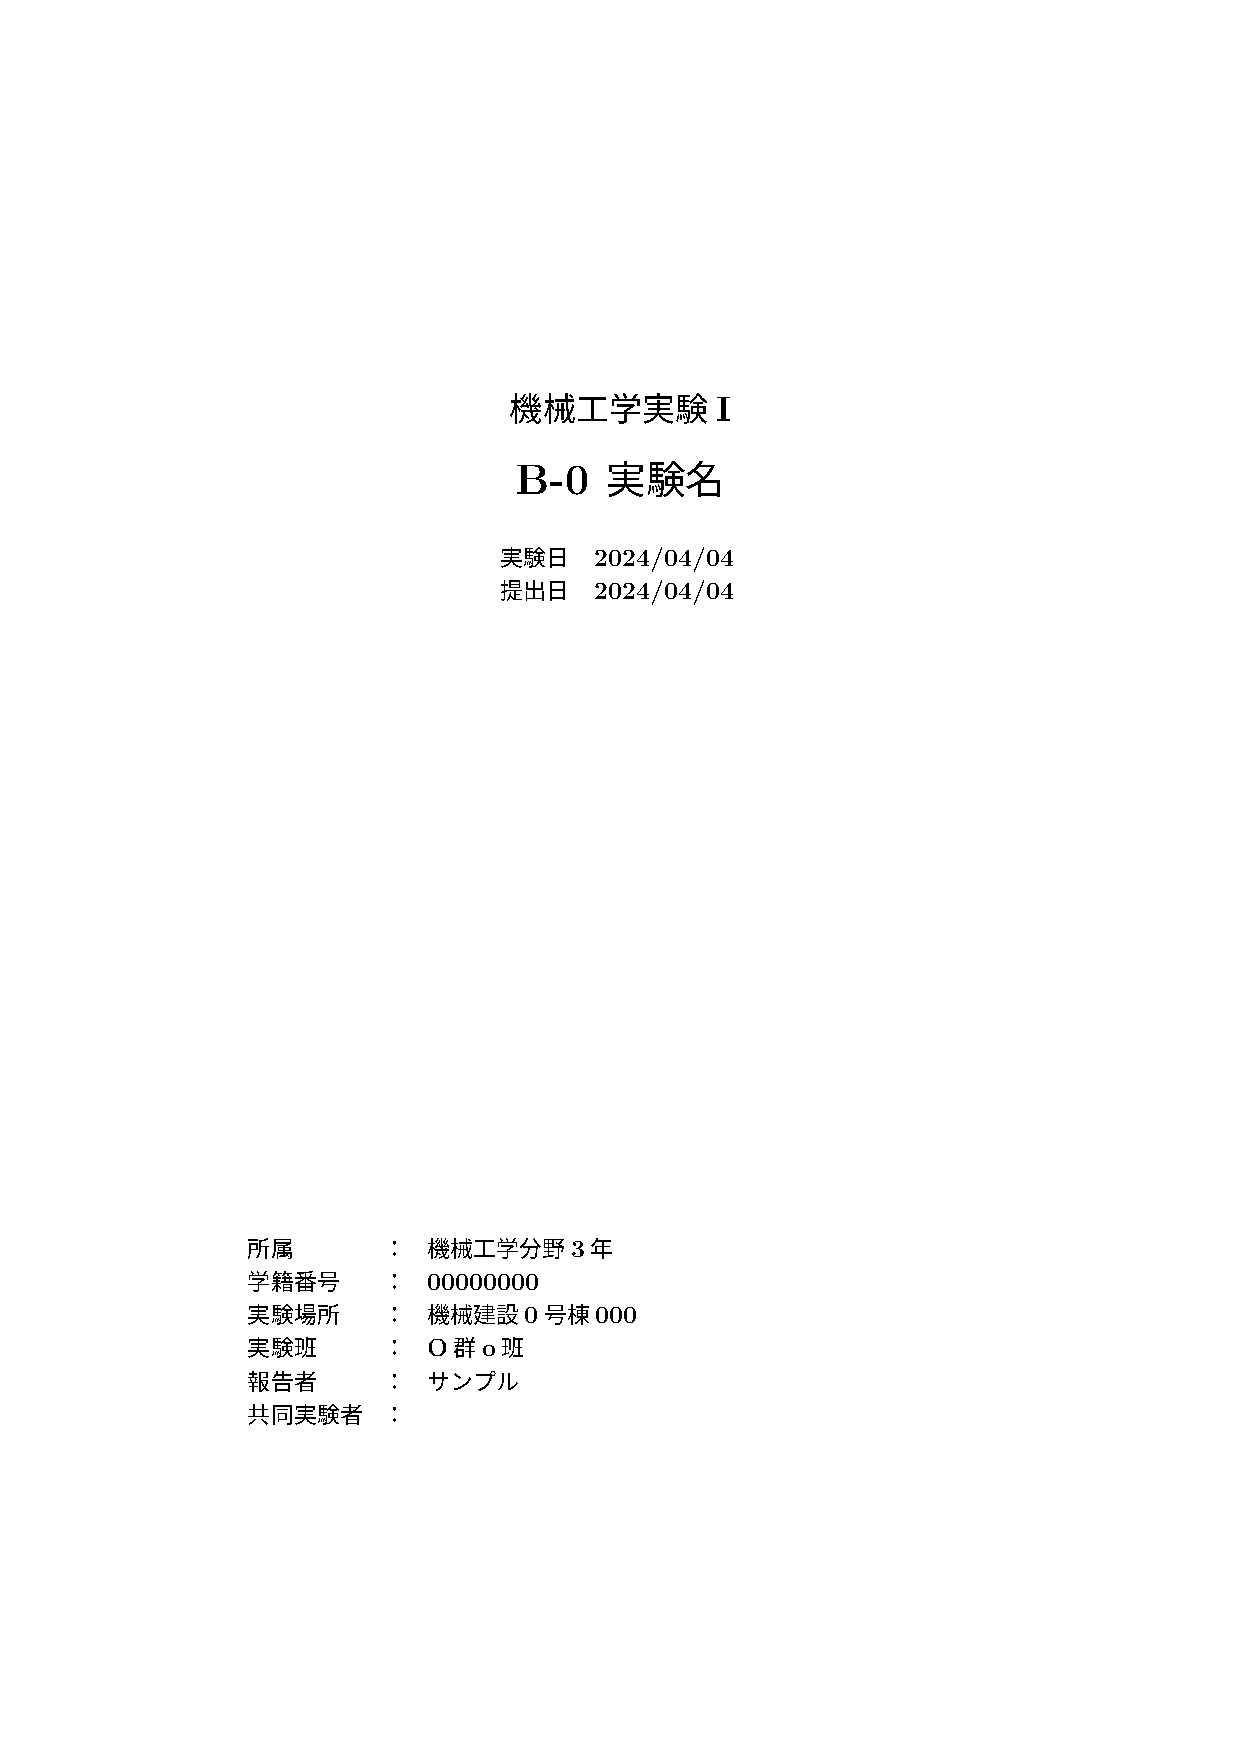
\includegraphics[width=40mm]{fig/sample.png}
\caption{サンプル画像}
\label{fig:sample}
\end{center}
\end{figure}

\begin{table}[htbp]
 \caption{表のサンプル}
 \label{tab:sample}
 \centering
  \begin{tabular}{cc|c}
   \hline
	inu & neko & niwatori \\
   \hline \hline
	dog & cat & chicken \\
	わん & にゃー & こけこっこー \\ \hline
  \end{tabular}
\end{table}

\begin{itemize}
	\item 箇条書き1
	\item[pro] 箇条書き2
	\item 箇条書き3
\end{itemize}

\begin{thebibliography}{99}
\small{
    \bibitem{neko} 参考文献です
}
\end{thebibliography}

\end{document}